%Chapter 3
\chapter{Theoretical Analysis and Approach}
\label{chap:analysis-and-arch}
This chapter presents an analysis of the system and literature regarding previous research.
It will segment different subsystems to separate the controlled system, the engineered system and the environment they are deployed in.
With the analysis done, we will have a clear understanding of relevant parameters and their interaction.
Which will be the basis for a sensitivity analysis to determine the most impactful components.
From this the main goal of this work is extracted.
% Knowing the objective and the most influential elements enables us to map out a solution proposal.
Knowing the objective and the most influential elements enables us to prune the system description to our specific application.
And then sculpt the concept.
It also prepares us for the simulation brought fourth in chapter \ref{chap:simulation}.

% First introduce the system and what is important, so the reader understands current implementations.
% Then prune the system to sculpt our concept.

% This chapter will give an overview over the state-of-the-art research.
% It examines the impact of 

% This chapter shall define the system and its boundaries.
% Define the goal of this work.
% This chapter will uncover the problem we are trying to solve.
% What it is we are trying to achieve.
% Then analysis of state of the art solutions.
%
\section{System Analysis}
\label{sec:system-analysis}
To design a solution, we must first know the structure of the problem. %and establish some terminology.
For this we need to get a tangible definition of the term system.
% For this we need to get more tangible with the term system.
% To break down, we must first know what a system is.
% A system might be defined in different ways.
% There exist different definitions of a system.
% There exist different definitions for what a system is.
For the engineer, it can be described as a collection of elements with properties of interest @schmitt2019.
Following this definition, we need to identify the systems' constituents.
And then analyze what about them is important to us.
% So let us first break down the different parts.
The next section will break down the different parts.
% When we have an overview, we review existing systems.
% So what are the constituents, and which attributes need to considered?
% We will define this by the necessary functions which a system like this needs to fulfill.

\subsection{Partitioning}
\label{sub:partitioning}
The primary classification is to distinguish between controlled system, engineered system and context.
The plant is the basis of the \textit{Controlled System}.
However, it is not possible to manage it directly.
% It can only be placed into an environment which 
We need to interface with its environment to affect these green lifeforms.
This environment is further divided into leaf and root surroundings, since they require different conditions.
Apparent from their different situation in nature.

Going back to the fundamentals of \ac{cea}, the \textit{Engineered System} is composed of three parts.
Illumination, irrigation and the atmosphere control.
They cater to the different needs of the plant.
Atmosphere control and illumination interface with the leaf environment, while irrigation takes care of the root system.
Together the controlled system and the engineered system make up, what we will call a 'farm'.

These parts are embedded into a greater \textit{Context} they need to operate in.
This is where this work diverges from previous concepts.
In the past, the field has tried to shield the farming context from outside influences.
Less exchange to the environment means a very high level of consistency and independence.
As we will see in the analysis of commercial farms (\ref{par:prop-ener-commercialfarms}), this approach has not proven successful though.
This is why this work embraces the context it operates in.
Seeing it not as a hindrance but as an opportunity for synergy.
As introduced before, this work places the farm on building facades. % we want to green facades.
Two different domains reveal themselves in this context.
The building insides and the city environment.
The \textit{City} in this work is classified as everything surrounding the envelope of the farm.
Therefore, the outside world with weather and the suns' radiation is integrated here and enables a hybrid approach to plant cultivation.
Part utilization of natural resources and part artificial optimization of the environment.
Similar to how greenhouses operate already. 
The interface to the \textit{Building} is novel. %directly leads to insulation
Potential for insulation naturally comes to mind, which provides a big benefit not exhausted in this work.
We will only evaluate insulation performance.
Energy savings for the building brought about by this choice are not considered in the energy balance built up in later chapters.
 % but not yet add it to the energy savings achieved by our design.
% Only skimmed by evaluating insulation performance but not exhaustivily discussed.
% The energy savings are not even considered.
% The possibility of building insulation emerges naturally by this.

These are the general parts which comprise our concept.
In the next section we will delve deeper into their interactions.
They will make up the properties of interest which are still missing for our system definition (\ref{sec:system-analysis}).

\subsection{Properties of Interest}
\label{sub:prop-of-interest}

\subsubsection{Controlled System}
\begin{wrapfigure}{R}{0.4\textwidth}
	\includegraphics[width=0.4\textwidth]{img/system_analysis/controlled-system.pdf}
	\caption{The plant and its immediate environment.}
	\label{wfig:controlled-system}
\end{wrapfigure} 

Beginning with the system we want to control, we illuminate the interface between the plant and its environment.
The root system is relatively straight forward to manage.
We need to supply water and nutrients while cleaning out waste products.
These are modeled as mass flows.
Water and substances dissolved within it are named $\dot{m}_{\text{H}_2\text{O}}$ in this work.
The waste products are captured with $\dot{m}_\text{W}$.

Shifting up to the leaf environment, photosynthesis presupposes two mass flows as well.
Carbon dioxide $\dot{m}_{\text{CO}_2}$ moves from the air to the leaves, while oxygen $\dot{m}_{\text{O}_2}$ diffuses out to the atmosphere.
During nighttime these flows are reversed to accommodate cellular respiration.
This is however not everything happening at this interface.
Most of the water taken up by the roots is actually not used in photosynthesis at all.
The plant uses it to carry nutrients up into its body.
This movement is fueled by transpiration.
About \SI{95}{\percent} of the $\text{H}_2\text{O}$ is carried out to the environment this way \textcolor{Blue}{needs ref}.

Next, energy in the form of radiation is required.
The total radiation hitting the leave surface is characterized by $R_\text{T}$.
This incorporates the spectrum and intensity of the light.
% Depending on the source it is divided into \ac{par} and \ac{ppfd}.
With this we have captured properties which flow from one system to another in the targeted context.
% There is however also an informational
% These are however not the only attributes of interest.
Tough there are still additional attributes of interest.

As shown later in the \nameref{subsub:yield-analysis} there are two other features of the atmosphere we need to take a closer look at.
Air temperature $T$ and air speed $v_\text{A}$.
These are inputs to the yield model we will introduce in the \nameref{subsub:yield-analysis}.
They are not flowing from one system to the other in a physical sense. % in contrast to the other characteristics.
Instead, these are properties informational in nature.
A block diagram of the plant and its immediate environment can be seen in figure \ref{wfig:controlled-system}.
Mass flows are shown as solid lines, energy fluxes dashed and data flow as dotted lines.
Now that we have defined the objective of our inquiry, the next section will talk about its supervision.

% \paragraph{}
% \vspace*{-\parskip}

\subsubsection{Engineered System}
\label{subsub:engineered-system}
% The first part we can influence, is
\begin{wrapfigure}{R}{0.6\textwidth}
	\includegraphics[width=0.6\textwidth]{img/system_analysis/engineered-system.pdf}
	\caption{The technical system and its influences.}
	\label{wfig:engineered-system}
\end{wrapfigure} 

Following the partitioning, the first technical subsystem is illumination.
At first thought it seems like we can interface with the plant leaf directly here.
However, we only supply a certain \ac{par} / \ac{ppfd} to the environment.
The plant is free to use any amount of it and will actually close its stomata -- the pores enabling gas exchange -- in light stress situations \textcolor{Blue}{needs ref}.
Effectively caping the light it uses.
And so the artificial radiation $R_\text{A}$ flows from the light source to the leaf environment.
Any technological light source can not be \SI{100}{\percent} efficient, and consequently heat flow from losses is modeled with $\dot{Q}_\text{R}$.
Another influence we can take on lighting is to shade the plants from excessive natural lighting.
This is frequently done in existing greenhouses to prevent aforementioned light stress.
The amount of light passing through will be called $R_\text{S}$.
This can be unimpeded or diffused natural radiation by shading.

Next let us look at atmosphere control.
The mass flows $\dot{m}_{\text{H}_2\text{O}}$, $\dot{m}_{\text{CO}_2}$ and $\dot{m}_{\text{O}_2}$ introduced before can all be controlled discretely.
Water in the form of humidity is an important factor to control \ac{vpd} as introduced in the \nameref{sec:fund-cea}.
And elevated levels of carbon dioxide promote mass accumulation and therefore higher yields.
Oxygen is nonessential in our inquiry and is only distinguished to keep an equilibrium of elements in the leaf environment.
% Oxygen is not of big interest and is only distinguished 
% shown separately because of the importance of carbon dioxide and water.
Furthermore, air temperature is one of the important factors in the yield calculation later.
Thus, the atmosphere management needs to be able to govern heat flow to and from the environment with $\dot{Q}_\text{A}$.
As always in control systems there needs to be some form of feedback.
Sensors to capture the relevant properties temperature, air speed and mass concentrations for water and CO$_2$ are placed in the air volume.
Note that carbon dioxide is usually measured as a volume concentration.
But, it is easy to convert these two values via the density.
And so no distinction is made in this investigation.
% For our investigation it is more convenient to look at mass flows.
% These values can be converted via the density.
Water in the form of humidity can be measured both as a mass or volume concentration.
The sensor data is aggregated with the atmosphere control signal $S_\text{A}$.

% For irrigation, we describe the water flow with any dissolved materials and waste products as $\dot{m}_{\text{H}_2\text{O}}$.
For irrigation, we describe the water flow with any dissolved materials as $\dot{m}_{\text{H}_2\text{O}}$.
Different to the water mass flow from the root zone towards the plant, this includes the waste products.
This is because at this point the pure waste products of the plants will be dissolved and transported together with the water flow.
\ac{vpd} of the root control volume is fed back through the irrigation control signal $S_\text{I}$.
With this we have gathered an overview of the attributes needed to govern the controlled system.
Figure \ref{wfig:engineered-system} shows the influences the technical system takes on the plant and its surroundings.
Subsequently, the next section introduces the setting in which this farm is placed.
% will highlight the context of our system.

% Now we introduce the part we as an engineer have control over.
% On cloudy days, supplemental lighting.
% This artificial radiation is called $R_\text{A}$.
% Just as the natural radiation it captures spectrum and intensity.

% \paragraph{}
% \vspace*{-\parskip}

\subsubsection{Context}
As established before we divide the context into two domains.
First we examine the urban environment.
Natural radiation $R_\text{N}$ by the sun illuminates the city and therefore the farm.
We discussed before that this can be managed to a certain degree by shading our leaf environment.
So this illumination from the city domain interfaces with the corresponding control system.
% diffusing the incoming light.
% the illumination control by shading.
We still need an input signal for the light management.
It makes sense to choose the incoming illumination flux as our radiation control signal $S_\text{R}$.
Since it determines how much shade or supplemental light is needed.
Next the atmosphere control can interface with the city environment by exchanging air $\dot{m}_{\text{Air}}$.
This can be in the form of opening windows or a more complex interaction when processing air with \ac{hvac} units.
% Heat flow from the farm envelope to the environment or vice versa is not something we can actively control.
Apart from the material choices, heat transfer from the farm to the city $\dot{Q}_{\text{FC}}$ is not something we can actively control.
And so it is shown as an energy flux between the building and leaf environments.
Note that the name $\dot{Q}_{\text{FC}}$ does not imply a direction of flow.
This is already taken care of by the direction of the arrows.
Other than introduced in the fundamentals on \nameref{sub:heat-transfer}, $\dot{Q}$ only includes conduction and convection.
Radiation is separated from the other heat transfers because it is special in our application and already modeled with $R_\text{N}$.

The important interaction taking place between the farm and the building interior is also a heat transfer $\dot{Q}_{\text{FB}}$.
The full block diagram of the system can be seen in figure \ref{fig:system-definition}.
This gives a good overview of what parts and properties are interesting when designing a concept for this application.
However, interest does not automatically imply necessity.
Fully controlled systems struggle to be profitable as teased before.
% A fully controlled system is not what this work is after as this has failed in the past.
Engineering is oftentimes about making compromises, so we have to analyze which features of the system are the most relevant.
This will enable us to make the right concessions and focus on the most impactful characteristics.
% This will enable to put the focus on the most impactful ones.
These themes are the topic of the next section.

\begin{figure}[htbp]
  \centering
  \includegraphics[width=\textwidth]{img/system_analysis/context.pdf}
  \caption{System partitioning and important flows.}
  \label{fig:context}
\end{figure}

\subsection{Sensitivity}
The first part of this section will establish why the energy demand is an important attribute in this endeavor.
Then it will go deeper into which systems are the culprits for high power draw.
From this we will then formalize the main goal of this work, which is to minimize energy consumption.
Next the sensitivity of parameters influencing yield will be discussed.
This provides an understanding on which compromises are the least harmful to economic performance of the farm.
This constrains the main goal with an auxiliary condition.
Maximizing yield.
In the end the analysis lays the foundation for which parameters are free design variables.
And which are restricted by the application.

% The weight of the different properties are discussed in this chapter.

% Analyzing the important attributes will give us a clear view which parameters are free design variables.
% And which are constraint by other properties.

% This information is extracted from the objectives this work tries to optimize.
% Minimizing energy consumption and maximizing yield.
% \begin{itemize}
% 	\item Minimize energy consumption
% 	% \item Provide insulation
% 	% \item [Auxiliary condition] Maximize yield
% 	\item Maximize yield
% \end{itemize}
% These two goals are subjected to a sensitivity analysis in the following sections.
% This enables us to gain an understanding which parameters of the system are the most relevant.
% This helps us to identify the most relevant parameters.

% What elements have the biggest contribution to energy consumption?
% And what is the sensitivity of the elements to the yield output?
% Insulation will be evaluated but is no main design priority.
% There are elements consumed by the plant -- co2, water, light energy -- and there are ambient factors like air temperature and velocity.

\subsubsection{Energy Analysis}
\label{subsub:energy-analysis}
% Firstly this work looks into the state of existing commercial farms.
% This provides reason to divert from the current path the industry is taking.

% To be able to evaluate the energy impact of the different technical subsystems, we will look at current vertical farming system.

% Let us first examine current \ac{cea} and vertical farming approaches to get a better understanding of the solution methods and shortcomings.
% Current solutions try to achieve high degree of automation and full control over the environment.
% This results in high energy

% Companies such as ... and ... try to seperate the plants completely from the elements and control the environment they are in fully.
% This of course is great for reproducibility and quality.
% However as we will show later in chapter \ref{chap:analysis-and-arch} current commercially operating farms with this approch have one main problem.
% Energy consumption.

\paragraph{Commercial Farms}
\label{par:prop-ener-commercialfarms}
In recent years, hype surrounding vertical farming has slowed significantly.
2023 marked a \SI{91}{\percent} decrease in capital investment compared to the year before, according to Pitchbook.
% https://foodinstitute.com/focus/what-does-aerofarms-bankruptcy-signal-for-ceas-future/
Multiple commercial endeavors declared bankruptcy.
\textcolor{Blue}{How do I cite recent developments? Like companies going out of business?}
Especially in Europe where Energy prices surged in the last years.
One notable example is InFarm -- a Berlin startup which was able to gather significant funding.
Despite the financial backing, all European branches have seized operation.
They restructured and continue to function in the Middle East, where energy is less of a concern than water scarcity.
% They continue to function in the Middle East, but European branches have seized operation.
The company itself has cited high cost from energy consumption as the primary reason.
% https://www.infarm.com/news/note-from-infarm-s-founders-strategy-shift-and-profitability-at-infarm
A focus of the company was to diversify the crops which can be cultivated.
Exemplified by their efforts to grow wheat, a plant which has not been demonstrated in this setting before.

Aerofarms is another big player which recently filed for bankruptcy.
During this process they needed to refocus their efforts on their only profitable farm.
% They operate in the US and during this process needed to focus their efforts on only profitable farm.
% https://www.aerofarms.com/aerofarms-emerges-fully-funded-from-chapter-11/
% https://en.wikipedia.org/wiki/Controlled-environment_agriculture
% In general two trends are observable.
Both companies focused on a highly controlled and automated approach to farming.
This of course is great for reproducibility and quality.
But as happens frequently, tech companies want to optimize.
And since each plant can have drastically different requirements on the optimal condition, they invested heavily into R\&D.
Some amount of research is undoubtedly required to compete with traditional agriculture.
However, optimization is endless and only offers diminishing returns the further it goes.
It is easy to end up with an overengineered system.
% However, since most of the entrepreneurs in this field come from a tech background, they tend to
% But easily leads to overengineered systems.
The author of this work is a proponent of \acs{kiss} principles.
And so the most impactful factors should be considered first.
% Luckily nature mostly provides a non-hostile environment.
Nature is utilized to nurture the parts of plant care deemed less important.
% High investment cost and R\&D efforts are needed to compete

% The lessons which can be drawn from the abovementioned developments are as follows.
These are only a few examples, but they represent a general trend in this field.
Two lessons can be drawn from these economic field studies.
% From the examples presented above two lessons can be drawn.
Firstly it makes sense to focus on one profitable crop in the beginning and optimize for that.
Lettuce is chosen in this work.
It is a staple crop for the majority of farms and the most researched in this context.
Secondly \textbf{Energy consumption needs to be minimized significantly}.
This is the most important result of our investigation and constitutes the research objective for this work.
The next paragraph examines which systems provide the biggest leverage to achieve this goal.

% They tried to achieve a very high degree of automation.
% Comes with very high initial costs.
% Not enough return fast enough.
% Tech bros are the entrepreneurs trying to make this happen.
% Trying to solve all problems with technology.
% This is expensive.
% Oftentimes nature can provide a big contribution to the nurturing of the plant already.
% The author is a proponent of kiss principles in engineering.

% These developments do not provide deep insight into the problematic subsystems.
% However, it validates the foundational assumption to minimize energy need.

\paragraph{Research}
As depicted in figure \ref{wfig:engineered-system} the technical implementation consists of three main subsystems.
% But which has the highest contribution to energy consumption?
We will group energy consumers according to this classification.
Surprisingly there exists limited data on which part demands the most power.
This is because these farms come in a variety of different forms and sizes and the field is still evolving.
For example atmosphere control in the form of \ac{hvac} has high upfront investment cost.
This only makes sense when the operation reaches a certain scale. % and is responsible for a jump in power draw.
So not every farm will employ it.
% In contrast, illumination can be deployed very fine-grained.
The implementation of irrigation can take very different forms as well.
We introduced a few methods in the Fundamentals (\ref{sub:fund-cea-irr}), but there are many more with varying levels of complexity and therefore energy demands.
Additionally, requirements for different crops can skew the results one way or the other.
For example basil needs more light than lettuce and subsequently has higher power draw for this subsystem.
Furthermore the location of the farm is also a factor.
When located in a hot and dry climate, the air conditioning will behave very different from a cold climate in Sweden for example. 
Nevertheless clear patterns and trends are visible.

% https://doi.org/10.1016/j.agsy.2017.11.003
For our analysis, we chose two studies looking at lettuce cultivation in different climate conditions.
Figure \ref{fig:energy-sensitivity} shows the resulting energy requirements from @graamans2018.
\begin{figure}[htbp]
  \centering
  \includegraphics[width=\textwidth]{img/energy-sensitivity.jpg}
  \caption{Energy use per \si{\kg} dry matter in different climate conditions @graamans2018.}
  % https://doi.org/10.1016/j.agsy.2017.11.003
  \label{fig:energy-sensitivity}
\end{figure}
We focus on the bars labeled PF, for Plant Factory.
In contrast, GH stands for Greenhouse.
These farming methods were analyzed for Sweden (SWE), Netherlands (NLD) and the United Arab Emirates (UAE).
We will look closer at the Dutch data, since the climate is the closest to Germany.
As we can see the vast majority of electricity is used for illumination by \acp{led}.
The cooling for this lighting system comes in second and third is dehumidification.
Cooling and dehumidification are the realm of atmosphere control.
Irrigation is not considered in this study.

% https://doi.org/10.1016/j.applthermaleng.2023.122129
Another study @arcasi2024 analyzes the sensitivity for different amounts of lighting and temperatures.
Copenhagen and Naples were the closest locations to Germany examined in this paper.
They come to a similar conclusion as illumination consumed between 65 to \SI{85}{\percent} of electricity.
10 to \SI{20}{\percent} can be attributed to \ac{hvac} systems.
Once again electricity use of irrigation was not considered in this study.
However, a whitepaper by the Association of Vertical Farming @zeidler2017 and anecdotal data for example from iFarm suggests that the consumption is negligible.
They find that illumination together with air management make up 95 to \SI{98}{\percent} of the total energy demand of vertical farming systems.
% https://ifarm.fi/blog/how-much-electricity-does-a-vertical-farm-consume
In the further analysis, irrigation is assumed to be inconsequential for energy demand.

This knowledge now determines the main design choice of the conceptualization.
Illumination is by far the biggest contributor to electricity need and so natural lighting shall be used.
Now one could argue that a vertical farm like this would offer no advantage over traditional greenhouse cultivation.
However when looking at the energy consumption data for greenhouses (GH) in the Netherlands (NLD) shown in figure \ref{fig:energy-sensitivity}, we can see that the power demand largely originates from heating.
The solar energy is supplied by the sun and does not need to be taken into account.
High power draw from heating makes sense in a greenhouse context.
The advantage of this cultivation method is to extend the growing season.
So in colder months it needs to be kept warm artificially.
However, a greenhouse is surrounded by badly insulated glass.
Furthermore, it has a wide interface for heat loss to the ground.
When placing the farm on the side of buildings, a distinct advantage emerges.
One of the big outside surfaces is no longer exposed to heat loss.
Instead, the building now provides heat gain to the farm.
Room temperatures humans are comfortable with are usually around 18 to \SI{21}{\degreeCelsius}.
Higher than what lettuce needs to grow.
The effectiveness of this will be shown later in the \nameref{chap:simulation}.
% More on the plants' specific temperature requirements can be found in the next section.
The interface for heat loss to the ground is minimized as well.
And of course other advantages like more regional production -- right inside the city -- remain.
% This knowledge now justifies one of the main design choices made in the conceptualization.
% To use 
Next, the factors influencing yield will be examined.
This will determine what subsystem shall retain optimal control and which will be no focus of this work.

\subsubsection{Yield Analysis}
\label{subsub:yield-analysis}
This section is still in construction.

When examining yield, we first need a definition of what is meant by that.
It depends largely on the crop under investigation.
The fruiting body, roots, leaves or even whole plants can all be considered produce in different contexts.
As argued before, we chose lettuce as our crop.
For this food item, basically the whole plant can be sold and so yield will be roughly equivalent to weight.
The yield model implemented in the later chapters was first proposed by @van\_henten1994.
It measures yield by modelling dry weight of the plant.

To get a rough understanding which are the most prevalent factors to influence plant growth, we will analyze a prominent lettuce yield model.
% The inputs to this model are considered the most influential.
Its details are introduced in \nameref{chap:simulation}, for now only the inputs are examined.
These are \ac{par}, CO$_2$ concentration and air temperature and are taken to be the most influential factors in determining growth.
Of course other factors like air flow and humidity are also essential to the health of the crop.
These are however assumed to stay in a reasonable range due to natural air exchange.
Just like in existing greenhouses.
% We will go off of what the yield model takes as input to determine which properties are of importance.
% The attributes going in are \ac{par}, CO$_2$ concentration and air Temperature.

A model can take the analysis only so far however.
If the temperature is \SI{-10}{\degreeCelsius} for example, lettuce will die.
The model happily will produce an output albeit very small.
In real life, lettuce grows comfortably in the range of 7 to \SI{24}{\degreeCelsius} and can survive temperatures even a little below freezing as anecdotal evidence suggests \textcolor{Blue}{check again}.
A temperature our system can provide as shown later in \nameref{chap:simulation}.
\textcolor{Blue}{Test model at -10C.}

% With the yield analysis we want to find out which input will produce the biggest difference in plant production.
% As mentioned before irrigation is a solved problem and this system is assumed to provide water and nutrients in an optimum manner.
% We will go off of a lettuce model to see which inputs the system deems important.
% The inputs are air temperature, CO$_2$ concentration and \acl{par}.
% It is difficult to make consistent statements about the influence of the parameters.
% Since the optima change for different combinations of inputs.

% % They describe the development of these two state variables in accordance to the inputs.
% The whole model is too extensive to be shown in this section and so only the top level equations are presented here.
% What is important for the investigation at hand are the dynamic inputs which influence this model.
% These are air temperature, CO$_2$ concentration and \acl{par}.
% In the implementation \ref{subsub:yield-model} the whole model can be seen.
% % For a more detailed discussion, please refer to the original paper.

% There are two ways to gain more information about a system.
% Running experiments in real life and simulating the system with a model.
% @van\_henten1994b followed up with a sensitivity analysis of the proposed model.
% They found that radiation has the highest influence very closely followed by CO$_2$ concentration.

% We choose one crop to optimize, however it is assumed that similar dynamics also play a role in other plant species.
% This is important, since this work tries to establish a general system.
% It does not aim to overfit to a specific crop type.
% This is why the energy impact of existing farms will be weighted more heavily than the yield analysis.

% Lettuce is chosen for a few different reasons.
% Firstly it is well suited to aeroponic cultivation \textcolor{Blue}{needs ref}.
% Secondly it grows quickly and consequently is more economically viable as for instance grain crops.
% This makes it one of the most used and researched crops in academic and commercial domains alike.
% Most of the different varieties of lettuce have similar growing conditions, hence no differentiation is made in this work.

% Now that we have a system we want to optimize, we need to analyze it more deeply.
% There are two ways this can be accomplished.
% Real plants in experiments and models in simulation.

% Temperature is a factor we need to control, to achieve an advantage over traditional agriculture.
% Otherwise, non-competitive.

% \paragraph{Experiments}
% For \textit{experiments} we look at available literature.
% Some paper suggests light spectrum has an even bigger impact than illumination magnitude.
% As discussed in the fundamentals we do not consider altering spectrum however.

% \paragraph{Simulations}
% For \textit{simulations} we implement a lettuce yield model proposed by Van Henten @van\_henten1994 in Modelica.
% The model is a system of nonlinear partial differential equations \textcolor{Blue}{check if actually right}.
% A follow-up paper @van\_henten1994b assessed the sensitivity of the input parameters.
% Their analysis showed the highest impact for radiation and CO$_2$ concentration.
% Radiation displayed slightly more effect on growth.
% This is mostly consistent with the experimental data discussed above.

% % Following the usual procedure in control theory, it would be best to linearize the system.
% % For linear control systems the methods are far more developed.
% % This is usually done when we have one operating point the system shall be kept in, limiting the linearization error.
% % However, our system shall grow, so we do not have a stable operating point.

% % Next plants are quite slow systems in the technical context.
% % Dynamics with a slow response and high dead time are generally not well suited to the methods of control theory \textcolor{Blue}{needs ref}.
% % This is why we will analyze the plant model with a more crude but still effective approach.

% % The specifics are discussed later in chapter \ref{chap:simulation}.
% % For now only the inputs and outputs are considered.

% \textcolor{Blue}{Instert picture of plant model.}

% Water and nutrient delivery is mostly a solved problem in moderate climates and specifically \ac{cea} contexts.
% Hence, it does not play a role in the yield calculation.
% The properties of interest in the atmosphere are temperature $u_T$ and CO$_2$ concentration $u_{CO2}$.
% For illumination, \ac{par} $u_par$ is considered.
% As is convention in control settings, inputs are labeled with $u$ and outputs with $y$.



% Plants come in a variety of different forms and varieties.
% Lettuce is chosen because it is the most researched in the field.
% To judge crop yield, which factors are important.
% We present a yield 

% To be able to judge which factors influence plant yield, we need
% As @esmaili2020 showed, highest variance for lighting, suggesting most impact to yield.

% To minimize energy consumption we have already found above 
% Lighting provides the biggest leverage.
% This was a priority when designing the system.
% Similar to greenhouse cultivation, natural light shall be used.
% But what impact does this have on insulation potential and maximizing yield.
% For insulation there is none.

% Let us analyze what elements enable us to maximize yield.
% Yield is produced by the plant, so let 
% For this we will introduce the Yield model for lettuce.
% \textcolor{Blue}{Input block diagram plant model and interactions.}

% Water and nutrient delivery is mostly a solved problem.
% This is why it is not taken as an input to the yield model.
% We will deploy an aeroponics system as reasoned in the fundamentals \ref{sub:fund-cea-irr}.

% The Energy Analysis \ref{subsub:energy-analysis} has shown that illumination in this context takes the highest amount of resources.
% The optimal lighting conditions can be achieved with reasonable complexity increase.
% One reason to optimize the lighting.

% For the atmospheric conditions
% For greenhouses, common practice is to elevate levels but keep windows open.
% As this work is in the context of sustainability, it is not considered supplementing CO$_2$.

% From the first point we can deduct t

% We will define this by the functions the system needs to provide.

% So what exactly is it this work tries to achieve and what are relevant properties?
% On a high level
% This work wants to demonstrate the feasibility of a system.
% This work wants to advocate, that greening the future city environment and making food production more resilient and better for the climate can be combined.
% It shall be determined if it makes sense to put plants on buildings.
% We want to take care of a plant.

% The plant is a system we can not control directly.
% However, indirectly there exists significant potential to optimize the plant environment.

% Define plant system.

% Definition System.
% To understand what is needed of a system we first need to define its boundaries.
% And interactions with adjacent systems.
% Context in which it is situated.
% Define scope which we can control.

% Yield model highly nonlinear.
% Difficult to analyze.
% Additionally, very slow systems with dead time basically impossible to control via classic control theory \textcolor{Blue}{needs ref}.

% For humidity / vpd, there could be no data found comparing the sensitivity to the other parameters.
% It is assumed that enough air exchange will happen from the farm to the outside air to achieve reasonable growth.
% This is what happens in greenhouses anyway.

\subsection{Conclusions from the analysis}
\label{sub:conc-analysis}
The energy analysis showed that we need to focus on lighting to minimize energy consumption.
As a result the suns' energy will be utilized.
From the yield analysis we gathered that the radiation has the biggest impact on yield.
% The extent of this lead depends on the source of the information.
Lighting thus is again the focus for our inquiry.
From this follows that the illumination system should supply the optimal \ac{ppfd} and accumulated \ac{dli} to the plant.
% The size of leverage difference is slight to significant depending on the source of the information.
In the contrary it means that the atmosphere control will be significantly cut in its competence.
The ability to precisely control CO$_2$ and humidity is not examined in this work.
This also makes sense from an economic standpoint as \ac{hvac} systems are quite costly.

From these conclusions, a new system description specifically for our implementation is presented in figure \ref{fig:system-definition}.
It is slightly different to the system design proposed before.
But more relevant to the concrete application in this work following the results of the analysis. %now only shows the parts which actually will be implemented.
The atmosphere control will no longer distinguish between mass flows of different molecules.
Instead, we accumulate them together to the mass flow $\dot{m}_{\text{Air}}$.
We also do not consider control for the air temperature, thus the heat flow is removed from the atmosphere control.

% From the yield analysis the result was that again we need to focus on the lighting.
% As a result we provide a lighting system for the farm to supply optimal \ac{dli} to the crop.
% Additionally as \ac{hvac} systems are expensive compared to \acp{led} -- another reason to not focus on atmosphere control for now.

% The last section defined the system in question clearly.
% It showed the most impactful parts.
% With this knowledge, we can prune the system description to arrive at our concept.
% It is pretty similar to the system design proposed before but now only showing the parts which actually will be implemented.
% The atmosphere control will no longer distinguish between the mass flows of different elements.
% Instead, we accumulate them together to the mass flow $\dot{m}_{Air}$.
% As we also do not consider control for the air temperature, we remove the heat flow from the atmosphere control.

\begin{figure}[htbp]
  \centering
  \includegraphics[width=\textwidth]{img/system_analysis/system-definition.pdf}
  \caption{The full control system description specialized to the application.}
  \label{fig:system-definition}
\end{figure}


\section{General Concept}
\label{sec:concept}
From the system definition (\ref{fig:system-definition}), we have a clear picture on the electrical and control systems necessary.
However, there exists quite a bit of engineering and logistics necessary so support this function.
These will be specified in the next section.
A general architecture of the system is presented which incorporates the results already established.
Then a concrete implementation path for the power system is presented to go off of for our specific example unit and simulation.
% A power architecture will be designed and presented enabling us to later 

\subsection{Functional Approach}
\label{sub:func-appr}
For a complete realization there exist secondary functions which need to be fulfilled additionally to the main control.
For example an atmosphere management hardly makes any sense when there is no envelope to keep air in a separate control volume.
Additionally, we need to supply energy to the systems and provide a structure to mount the farm to a building.
From the chosen crop -- lettuce -- there also follows a high turnover rate.
It is usually ready to harvest in four to six weeks.
Therefore, easy mount and demount of the planting arrays is necessary.
These supporting components to the system as well as the tasks of the main system will be formalized and presented as functions.
A precise formulation of these will aid in defining our scope. %, extracted from the analysis.
The roles our concept shall serve are listed below.
They break down the goals of minimizing energy consumption and maximizing yield as well as concretize what additional infrastructure is needed to achieve these objectives.
\begin{itemize}
	\item Supply optimal lighting conditions.
	\item Provide a reasonable temperature range to grow lettuce.
	\item Maintain sufficient air exchange to keep CO$_2$ and humidity levels in check.
	\item Sustain optimal water and nutrient delivery.
	\item Serve a mounting structure to be able to retrofit the system onto buildings.
	\item Provide transportation mechanism to easily harvest and replant the crops.
\end{itemize}

Moreover, defining what is out of scope often helps to make the main requirements easier to understand.
Functions which shall \textit{not} be implemented are as follows.
\begin{itemize}
	\item Provide optimal CO$_2$ concentration.
	\item Maintain optimal temperatures.
	\item Illuminate with optimal light spectrum.
	\item Offer optimal humidity levels.
\end{itemize}

This formalization provides a better understanding of the extent for this work.
From this we will build the architecture in the next section.

\subsection{Structural Architecture}
\label{sub:stru-arch}
The reason we formulate a structural architecture is to convey the general idea for our implementation.
This shall serve to give the reader an understanding of all the parts required to realize the concept.
To convey this type of system information SysML provides a standardized framework.
% Subsequently, it is chosen for this task.
% SysML offers a standardized way to convey system information.
It implements an informational model as well as a visual representation for systems engineering.
Subsequently, it will be used to present the concept.
There are different diagram types, of which only structural diagrams are employed in this work.
More specifically the \ac{ibd} is used.
This type of diagram describes a systems constituents.
These are pictured by rectangles.
Connections have a diamond shape on the part which is deconstructed.
The arrow points to the smaller components.
For a full system design, there are a myriad of diagram types available in SysML.
However, this work cannot provide a full system design and therefore only uses this one diagram type.
This will enable us to describe the proposed concept.
% From the main system description and the other secondary functions the system needs to provide, we can now extract the structural architecture more easily.

For the structural architecture we will go off of two things we developed so far.
Firstly the control system following our system definition (\ref{fig:system-definition}).
Secondly the functional architecture defined in the previous section.
Detailing functionality of main and support systems.
This distinction is a bit arbitrary but needs to be made at some cut-off point.
For example the control system description could include a system for planting and harvesting, since it is technically needed to convert the plant to economic output.
However, in this way the system description grows to large.
And so main functions and supporting functions are distinguished.
The order these components are introduced roughly follows a spatial line, starting from the building and attaching the systems outward to the city.
% For comprehensibility’s sake, we will present the architecture going spatially from the building to the outside.
In the final diagram (\ref{fig:architecture}) this is represented with more foundational components to the left of the figure.
The introduction of these blocks will follow a particular pattern.
Firstly the main function of the block is presented.
Then other requirements for this system are laid out and the structure presented in written and visual form.
If useful a 3d model is presented to visualize the architecture with a tangible example.

% Also, a 3d model is presented to make the architecture more tangible.
Following the theme of going from the building to the outside, let us first get a look at the building in question.
It can be seen in figure \ref{fig:3d-building}.
It shows a 3d model implemented in Blender.
The pictures for the building faces were made by the author.
The 2d plane representing the ground was taken from a satellite image in Google Maps \textcolor{Blue}{am I allowed to do this?}.
The 3d geometry data is taken from \textcolor{Blue}{needs ref}.
\begin{figure}[htbp]
  \centering
  \includegraphics[width=\textwidth]{img/3d_model/building.png}
  \caption{3d model of the EEI-tower.}
  \label{fig:3d-building}
\end{figure}

\pagebreak

\subsubsection{Load-Bearing Structure}
\begin{wrapfigure}{R}{0.4\textwidth}
	\includegraphics[width=0.4\textwidth]{img/architecture/load.pdf}
	\caption{The load bearing structure.}
	\label{wfig:load}
\end{wrapfigure} 
With this in mind, let us first discuss the mounting structure.
Its function is to provide a load bearing foundation for any other subsystem to attach to.
\paragraph{Requirements and Structure}
One point to note is that the system shall be retrofitted to existing buildings.
Therefore, it should be self-contained in supporting its own weight.
Moreover, building faces are very diverse.
Consequently, the load-bearing infrastructure needs to be closely matched to the existing building.
It provides the interface for other subsystems.
% These are defined later.
The mounting for \textit{Pipes}, \textit{Panels} and \textit{Transportation System} are part of different components and are defined later.
% Pipes are for the bigger water system, Panels represent basically the root environment and its direct control with irrigation.
% The transport system 
% It shall not damage the facade or other structures on the existing buildings.

\subsubsection{Water System}
\begin{wrapfigure}{R}{0.6\textwidth}
	\includegraphics[width=0.6\textwidth]{img/architecture/water.pdf}
	\caption{The water system mixing and delivering the nutrient mix.}
	\label{wfig:water}
\end{wrapfigure} 
The next system that would need to be installed is the water system.
% It does not have a direct equivalent in our system description from \ref{}.
It is not equivalent to the irrigation in our system description from \ref{fig:system-definition}.
There we already presupposed the water and nutrient mix to be prepared and available to the irrigation system.
The water system will take care of this task.
Distributing the solution across the whole farm, as well as preparing it with optimal \ac{ec} and pH-levels.
% This mixture is then supplied to the panels.
\paragraph{Requirements and Structure}
The water supply needs to interface to the actual irrigation system.
This is illustrated by the part \textit{Connection for Panels}.
A water tank stores and supplies the \textit{Nutrient Mix}.
We later reason that the energy of the farm should be supplied by a \ac{pv} array.
With this knowledge it makes sense to position the water tanks on the roof of the building.
During the day solar energy can be used to pump and prepare the water mix.
And during nighttime gravity will provide water pressure to the system.
% As discussed later we will also utilize a solar array.
% It makes sense to pump the water during the day up to a water storage on the roof of the building.
% During nighttime gravity will provide water pressure to the system.
% Needs to prepare the nutrient supply.
A connection to the water system of the building is also conceivable.
This would need to process and monitor the nutrient mix either on the roof aswell -- to keep the water pressure -- or distributed at every floor.
To keep the retrofit concept simple and minimally invasive, a separate water circuit is proposed here.
To facilitate the water flow \textit{Pipes} and a \textit{Pumping System} is needed.
Furthermore, drainage for the \textit{Waste Products} as well as treatment is required.
% \textcolor{Blue}{Need to fit to presentation pattern.}
% Water tanks to store water.
% Pumps can run during the day when solar output available.

\subsubsection{Plant Panels}
% \begin{wrapfigure}{R}{0.3\textwidth}
% 	\caption{A plant panel stocked with lettuce plants.}
% 	\label{wfig:panel-full}
% 	\includegraphics[width=0.3\textwidth]{img/3d_model/3d-panel-full.png}
% \end{wrapfigure} 
For the actual irrigation system we will go into a little bit more depth.
The concept of the plant panel will ensure optimal water and nutrient delivery to individual plants.
\paragraph{Requirements and Structure}
The general idea is to modularize the whole system.
Providing a standardized platform for any building.
% The idea is to have a slim system to house the plants' roots.
One could imagine around three different sizes to best accommodate the space available on the facade.
Additionally, they provide smaller compartments to take care of.
This is important to stop the spread of plant diseases.
As well as provide fine-grained control of the plants.
Ideally you would want a control system taking care of every plant individually.
This however entails high cost and a trade-off needs to be made similar to the lessening of automation in \ac{cea}.
The modularization makes it possible to stagger planting and harvesting.
Additionally, the system needs to be slim to not require big open spaces in front of the building.
With these requirements we arrive at a panel like architecture.
Now that we have a rough outline of what we want the system to look like, we can take a closer look at how and what shall be implemented.
As discussed before, the panels shall take the role of irrigation.
For this they need to provide a closed volume for the root zone.
This is the main structure of the presented panels -- a container segregating the root environment from the rest of the farm.
As detailed in \ref{sub:fund-cea-irr} the system will use aeroponics.
This of course can be exchanged for any other hydroponic strategy inside the panels.
For example one could imagine \ac{nft} channels inside the same panels.
For the aeroponic system, an ultrasonic piezoelectric vaporizer is placed in a water-filled upper part of the panel.
Which can be seen in figure \ref{fig:3d-panel} (c) illustrating the inside air volume.
There, a pipe is shown to house the vaporizers.
This sustains a fog which provides \textit{Moisture and Nutrients} to the root environment.
This technology of course is not perfect.
% \begin{wrapfigure}{R}{0.3\textwidth}
% 	\caption{The inside volume of the panel.}
% 	\label{wfig:panel-inside}
% 	\includegraphics[width=0.3\textwidth]{img/3d_model/3d-panel-inside.png}
% \end{wrapfigure} 
% \begin{wrapfigure}{R}{0.3\textwidth}
% 	\caption{A panel without any plants present.}
% 	\label{wfig:panel-empty}
% 	\includegraphics[width=0.3\textwidth]{img/3d_model/3d-panel-empty.png}
% \end{wrapfigure} 
Anecdotal information suggests that these vaporizers will crust up with salts dissolved in the water over time.
They also heat up the root zone.
Root zone temperature is considered separately from the main air temperatures in some studies.
Suggesting that it might be an impactful parameter in plant growth and health.
This work did not analyze this further though as the general concept of the panel can be the platform for different irrigation strategies.
The root volume is controlled according to the system design (\ref{fig:system-definition}) with a feedback control.
A \textit{Humidity} and \textit{Temperature} sensor supplies the \ac{vpd} information to a \textit{Controller}.
The panel should also be able to get rid of the waste products exuded by the plant root.
An \textit{Outflow} is provided by the concept.
The panel structure holds all the different parts interacting with each other.
The architecture is presented in figure \ref{fig:panels}. 
And a 3d model mounting the panels to the building can be seen in figure \ref{fig:3d-panels-on-building}.
\textcolor{Blue}{Rename elements in architecture to fit with names in the text.}

\begin{figure}[htbp]%
    \centering
    \subfloat[\centering ]{{\includegraphics[width=0.3\textwidth]{img/3d_model/3d-panel-full.png} }}%
    \quad
    \subfloat[\centering ]{{\includegraphics[width=0.3\textwidth]{img/3d_model/3d-panel-empty.png} }}%
    \quad
    \subfloat[\centering ]{{\includegraphics[width=0.3\textwidth]{img/3d_model/3d-panel-inside.png} }}%
    \caption{3d models of the plant panels (a) fully stacked with lettuce, (b) empty, (c) open to expose the inside space for roots and nutrient fog.}%
    \label{fig:3d-panel}%
\end{figure}

\begin{figure}[htbp]
  \centering
  \includegraphics[width=\textwidth]{img/architecture/panels.pdf}
  \caption{The plant panels proposed by this work.}
  \label{fig:panels}
\end{figure}

\begin{figure}[htbp]
  \centering
  \includegraphics[width=\textwidth]{img/3d_model/3d-3-panels.png}
  \caption{3d model showing the plant panels mounted to the building facade.}
  \label{fig:3d-panels-on-building}
\end{figure}

\pagebreak

\subsubsection{Transportation System}
\begin{wrapfigure}{R}{0.5\textwidth}
	\includegraphics[width=0.5\textwidth]{img/architecture/transport.pdf}
	\caption{The transport platform eliminating the need for manual (de-)mounting.}
	\label{wfig:transport}
\end{wrapfigure} 
As mentioned before the system needs to transport the panels to and from the facade.
This is again a supporting function not found in the main control system description.
\paragraph{Requirements and Structure}
The farm needs to \textit{Mount and Demount} the panels to and from the load bearing structure (\ref{wfig:load}).
Then it needs to move the panels across the face of the building to a base where they can be harvested and restocked with fresh plant shoots.
It should also be as low profile as possible.
From this the concept of a wire-hung \textit{Platform} is developed.
It consists of a main structure responsible for (un-)loading the panels and necessary \textit{Control Infrastructure}.
A \textit{Hanger Assembly} made up of steel wires supports the weight of the construction and moves it around the farm.
The structural architecture of the block can be seen in figure \ref{wfig:transport} while a closeup of the transportation system is shown in picture \ref{fig:3d-transport}.

\begin{figure}[htbp]
  \centering
  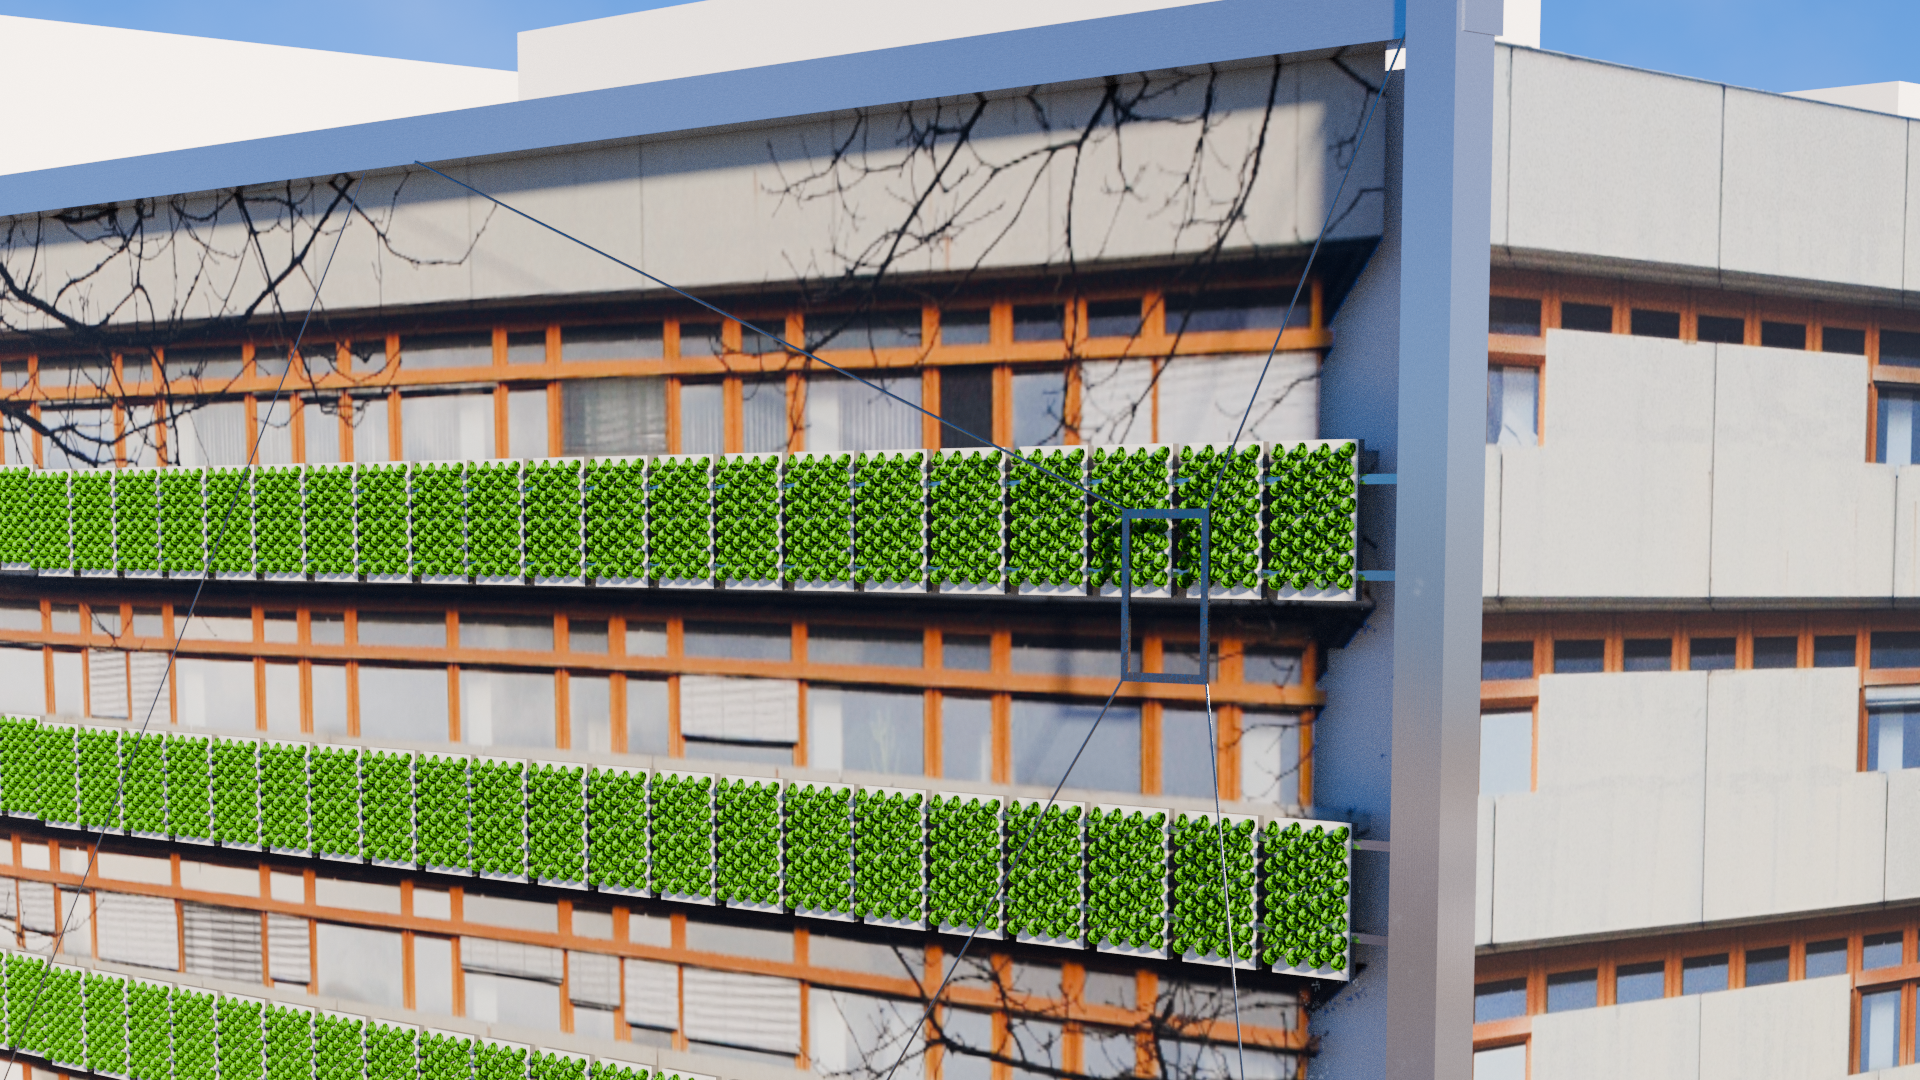
\includegraphics[width=\textwidth]{img/3d_model/3d-4-transport-closeup.png}
  \caption{3d model showing the general idea of the transport platform.}
  \label{fig:3d-transport}
\end{figure}

\subsubsection{Energy System}
Next a system needs to provide power to all the electronic subsystems.
This can be expanded into energy storage and generation as well.
The reason for this is to counteract the energetic impact generated by the farm as much as possible.
This is done because -- as mentioned before -- the German electricity mix is far from carbon-neutral.
Consistent with our motivation to make food production more green, a solar array is considered to generate energy.
As we will show later in chapter \ref{chap:simulation} it may even be possible to completely nullify the energy consumption with this procedure.
\paragraph{Requirements and Structure}
As we want to employ \ac{pv} it makes sense to rely on \ac{dc} components wherever possible.
The biggest energy consumers are the lighting fixtures.
% \acp{led} are chosen for their high efficiency, excellent service life and granular control of spectrum.
\acp{led} are chosen for a few reasons closer illustrated in the \nameref{subsub:climate-control}.
They need to be supplied by \ac{cc} which usually is more easily converted from \ac{dc} circuitry as well.
% So the energy system needs to provide a \ac{dc} power circuit to all the components.
% The biggest consumer of power, the \acp{led} need \ac{dc} and therefore the main circuit is chosen to be \ac{dc}.
% This fits in well with a battery and solar array.
% Next the system shall generate energy by a solar array.
% The reasons for this are mentioned above.
The chosen irrigation strategy is highly dependent on active control, otherwise the plant roots dry out quickly.
So we need to store energy to be resilient to power outages.
Hence, an energy storage is needed.
Batteries are chosen for this task as they are the most comfortable way to store electrical energy.
The system shall also provide a connection to the grid.
This is because the energy generation and consumption in our farm show a negative correlation.
When the sun is shining, the \ac{pv} installation will provide a lot of energy, while not much energy is needed for supplemental lighting.
Conversely, when there is little sun, we have a high energy demand from the \acp{led}, while not much energy is generated.
So from these requirements we separate the system into the three parts \textit{Energy Generation}, \textit{Energy Storage} and \textit{Energy Distribution} as seen in figure \ref{fig:energy}.

\begin{figure}[htbp]
  \centering
  \includegraphics[width=\textwidth]{img/architecture/energy.pdf}
  \caption{The energy subsystem.}
  \label{fig:energy}
\end{figure}

\subsubsection{Climate Control}
\label{subsub:climate-control}
The function of optimal light and reasonable atmosphere control is compounded into one part, the climate control.
\paragraph{Requirements and Structure}
The lighting system as discussed before needs to provide a structure to \textit{Shade from excessive Light}.
This is proposed to be simple semi-transparent cloth similar to existing greenhouses.
It would be deployed comparable to an awning.
To not block the view of the people inside the building.
Next if there happens to be little sun, we need to supply \textit{Supplemental Lighting}.
\acp{led} are chosen for a few reasons.
Their spectrum can be finely adjusted to facilitate photosynthesis exceptionally well.
They are comparatively cheap, efficient and therefore also do not produce a high amount of excess heat.
Furthermore, they offer class leading lifespans.
The amount of light entering the farm needs to be monitored and the shades and \acp{led} regulated with a \textit{Control System}.

For the atmosphere \textit{Control} we need to monitor the air volume and so \textit{Sensors} specified in section \ref{subsub:engineered-system} are employed.
\textit{Ventilation} is required.
This takes the form of a passive system in our concept.
Simple windows at the top and bottom of the farm will provide airflow.
They can be controlled according to the sensor inputs.
For the architecture we also consider \textit{Dehumidification}.
As plants evaporate water the humidity inside the farm will rise above average levels.
This may pose a problem for the building facade and air quality.
In our later inquiry and simulation it is dropped however as atmosphere control is not the focus of this work.
The internal block diagram can be seen in figure \ref{fig:climate}.

\begin{figure}[htbp]
  \centering
  \includegraphics[width=\textwidth]{img/architecture/climate.pdf}
  \caption{The climate control to take care of the leaf environment.}
  \label{fig:climate}
\end{figure}

\pagebreak

\subsubsection{Envelope}
\begin{wrapfigure}{R}{0.3\textwidth}
	\includegraphics[width=0.3\textwidth]{img/architecture/envelope.pdf}
	\caption{The envelope segregating the farm from the city environment.}
	\label{wfig:envelope}
\end{wrapfigure} 
The envelope provides the secondary function of separating the farm from its surroundings.
This is not formulated explicitly in the functions above.
Because it is inherent to have a separate environment if you would like to provide atmosphere control.
% This is quite primary as otherwise no \acl{cea} is possible.
\paragraph{Requirements and Structure}
As just discussed the envelope needs to provide a separation to the city environment.
This is accomplished by \textit{Self-Supported Framing} and \textit{Glazing}.
For this work we propose glass as it is durable and visually pleasing.
This is wrapped around the whole farm and building.
Not a requirement for our concept but another resulting function of this structure is the insulation.
One could imagine confining the envelope to the panels and therefore facade area.
When just covering the facade it would be best to separate the envelope and the insulation into two distinct parts.
This is because traditional insulation needs to be very close to the wall with little air movement.
For this work we chose to simplify this structure and therefore just encapsulate the building in a greenhouse shell.
This comes with the added benefit of insulating the window area, which usually is responsible for a high fraction of the heat loss of the building.
The complete architecture can be seen in figure \ref{fig:architecture}.
Note that this diagram only goes down to the second level of block definition.
This is done to make it more comprehensible.
A more detailed look at the components is already provided in the sections above.% show the more elaborate formulation of each constituent.
% It is cut-off at the second level of block definition, as otherwise it would become too unwieldy to present whole.
\textcolor{Blue}{Add 3d model of full farm}.

\begin{figure}[htbp]
  \centering
  \includegraphics[width=\textwidth]{img/architecture/architecture.pdf}
  \caption{The structural architecture of our farming concept.}
  \label{fig:architecture}
\end{figure}
\textcolor{Blue}{Switch climate control and envelope in full architecture.}

\subsection{Power System Architecture and Choice of Components}
\label{sub:power-arch}

% \subsubsection{Choice of Components}
As argued before we employ a battery and \ac{pv} installation.
It makes sense to rely on \ac{dc} devices wherever possible.
These parts will be detailed more diligently in the following part.
We will go through the components in order of their electricity consumption in traditional \ac{cea} systems.
Then \ac{hv} and \ac{lv} circuits are introduced to connect the system together.

\subsubsection{Illumination}
For shading one could imagine two types of deployment.
Linear Actuators extending the cloth of the awning or rotary motors rolling up the fabric.
Because of the prevalence of ordinary rotary motors, they are chosen for this application.
Now the choice presents itself if traditional \ac{dc} or \ac{bldc} motors are deployed.
This work chooses \ac{bldc} motors across the board for small to medium actuation tasks.
They are available in a wide variety of power classes, offer high efficiency and long operational reliability.
The general idea for deployment is to use one motor for multiple awnings.
As speed is not of importance, we can use a transmission -- of for example 1:100 -- to drive all awnings on one floor.
We choose the \textit{PBL42-15 48V} motor by Parvalux.
It offers a continuous torque of \SI{0.063}{\N\m}, resulting in around \SI{6}{\N\m} after the transmission.
This work does not verify the exact value by calculation, nevertheless it should be plenty for this application.
The transmission ratio can also still be changed later if not suitable.
The motor requires a \SI{48}{\V} \ac{dc} connection.

Next up we discuss the artificial lighting.
There exists a very large variety of \ac{led} lighting products specifically for horticulture applications.
\textit{300 XT EVO MIXED LM301H 3500K+4000K+660nm+730nm KIT} from LED-Tech is chosen because it offers full spectrum light.
This is important because we want white illumination as discussed before.
The spectrum is still optimized for photosynthesis, emitting light peaks at around \SI{440}{\nm} and \SI{660}{\nm}, close to the optimal absorption wavelength of chlorophyll a \& b.
It uses LM301H \ac{led} diodes manufactured by Samsung which offer class leading efficiency.
Additionally, LED-Tech provide great documentation showing the exact spectrum and light output for any of their \ac{led} modules and different supply currents.
When driving the chosen panel at \SI{2.1}{\A}, it outputs \SI{218.28}{\umol\per\s}.
Pretty close to the \ac{ppfd} of \SI{200}{\umol\per\square\m\per\s} which is optimal for lettuce cultivation.
\textcolor{Blue}{Did I already introduce this?}
So one of these panels is deployed per square meter.
As introduced before \acp{led} need to be run with a \ac{cc} source.
It is proposed here to deploy one driver per \ac{led} module.
This work does not go further into the topology of these circuits.
% However, it might be more economically feasible to group multiple panels together for one current source.
Next we will talk about the actors needed for the chosen atmosphere control.

\subsubsection{Atmosphere Control}
As argued before, the atmosphere control implemented here is confined to a passive system.
This is realized by opening and closing windows.
Again the same \ac{bldc} motor as for actuating the awnings with a higher transmission ratio of 1:200 is chosen.
A simple rack and pinion gear combination is picked to open the windows.
The torque of \SI{12}{\N\m} is supposed to be enough to drive the windows per floor.
Windows are placed on the lower and uppermost floor to promote air flow.
The coming section introduces the pumping system.

\subsubsection{Water System}
For the irrigation circuit we propose a \ac{bldc} with a higher power rating by Lorentz.
They specialize in solar-powered pumps and are therefore perfect for our deployment.
Their \textit{PS2-4000} controller and \textit{ECDRIVE 4000} pump combo is able to supply the needed water flow rates to the building height.
As can be seen in their documentation.
The required flow will be simulated later in chapter \ref{chap:simulation}.
The controller takes a maximum voltage input of \SI{375}{\V} and transforms it to three-phase \SI{240}{\V} \ac{ac} for the motor.

\subsubsection{\ac{pv} Installation}

\subsubsection{\ac{hv} and \ac{dc} Circuits}
The system will make use of a \ac{hv} and multiple \ac{lv} circuits.
The \ac{hv} part orients itself to be  compatible with batteries of electric vehicles.
% Since this is a big market there exist a wide variety of offerings.
Following our motivation for a more sustainable and circular economy, this opens up the possibility to reuse old car batteries.
They usually provide a voltage between 350 - \SI{400}{\V}.
The industry aims for higher voltages in the \SI{800}{\V} range for more luxurious vehicles.
However, budget oriented options are posed to stay at the aforementioned voltages.
Our chosen water pump has a maximum input voltage of \SI{375}{\V} and so the lower end of around \SI{350}{\V} is chosen for the \ac{hv} circuit.
For the \ac{lv} part a \SI{48}{\V} circuit is chosen.
This is a common value in \ac{lv} power distribution networks.
However, because we have a lot of components, the power we need to supply is high.
This means we cannot simply rely on a singular \ac{lv} circuit.
The current would melt the wires.
As argued before, the employed \ac{led} modules run at \SI{2.1}{\A} per square meter growing space.
\SI{37}{\V} follow from this supply current according to the supplier website.
We group them in pools of fifty panels.
This results in a power draw of $50 * \SI{2.1}{\A} * \SI{37}{\V} \approx \SI{3.9}{\kW}$.
% The \SI{37}{\V} follow from the supplied current according to the supplier.
At the \SI{48}{\V} \ac{lv} distribution network this translates to \textasciitilde\SI{81}{\A} of current for one \ac{lv} circuit, which is still manageable.
As we have around \SI{500}{\square\m} of growing space, ten \ac{lv} converters are needed in the system to distribute the load between them.

The block diagram for the energy architecture can be seen in \ref{fig:power-architecture}.
Because we have a lot of duplicated components -- eg. ten \ac{lv} converters, 500 \ac{led} modules -- only one of these elements is shown at a time in the diagram.
The others are connected in parallel.

\begin{figure}[htbp]
  \centering
  \includegraphics[width=\textwidth]{img/power-architecture.pdf}
  \caption{The power architecture of our concept.}
  \label{fig:power-architecture}
\end{figure}

\section{Feasibility}
\label{sec:feasibility}
Lastly to judge the proposed system a number of metrics are introduced.
These serve to evaluate the feasibility of the concept.
% Feasibility in this work does not mean that a system like this definitely makes sense.
Feasibility in this work just wants to judge and evaluate the concept on a few different fronts.
% Metrics to evalute feasibility of the concept:
The metrics this work proposes, are as follows:
\begin{itemize}
	\item The energy consumption can be met through a solar installation covering at most the area on the roof.
	\item Yield can offset investment costs in a reasonable timeframe.
	\item The farm provides a measurable insulation increase in comparison with the 'naked' building.
	\item Acceptance of potential customers to put a greenhouse on the side of their buildings is present (not evaluated in this work).
\end{itemize}
These points will be picked up later in \ref{chap:results} to assess the outcomes of this work.

